




\subsubsection{NAT - Network Address Translation}

\begin{definition}{NAT (Port Mapping)} Port-basierte NAT (NAPT) {\tiny (Boomer Paranoia)}    
    \begin{itemize}
        \item Ersetzt private IP-Adr. durch public IP des Gateways/Routers
        \item Ersetzt private Port-Nr. des Hosts durch freie zulässige Port-Nr. des Gateways/Routers
        \item Mapping privater IP-Adr. und Port-Nr. zur öffentlichen Port-Nr.
                \\auch statisch möglich, aber nur Port-Nr wird übernommen
    \end{itemize}
    Problem mit NAT: Verletzung des OSI-Layer-Konzepts\\
    Um Port im TCP Header zu ändern müssen Daten im IP-Frame verändert werden 
    $\rightarrow$ Netzwerk-Funktion greift auf den Transport Header zu,
    IP-Adresse/Portnummer werden dabei verändert\\
        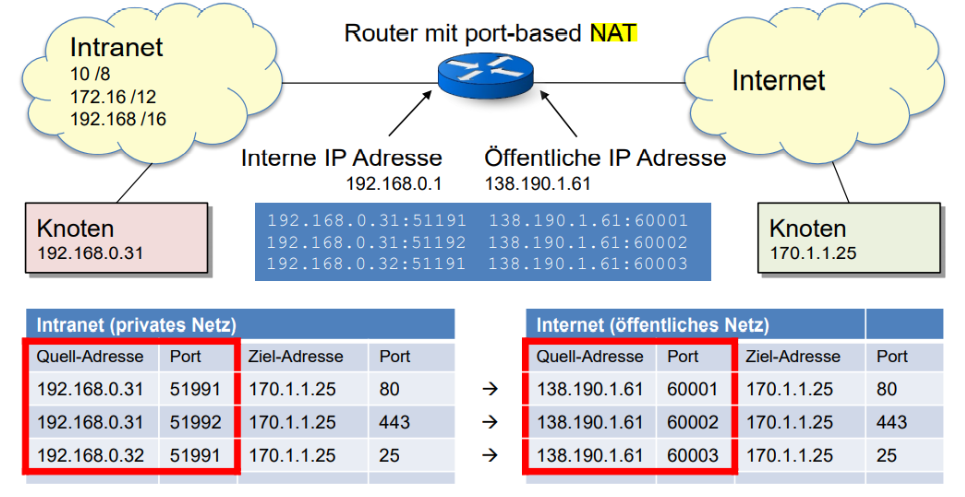
\includegraphics[width=1\linewidth]{images/NAT.png}
\end{definition}
\begin{remark}
    $\forall$ Hosts im privaten Netz 192.168.0.0/8: Default-Gateway 192.168.0.1
\end{remark}

\subsubsection*{Von A bis Z: Aufruf einer Webseite}

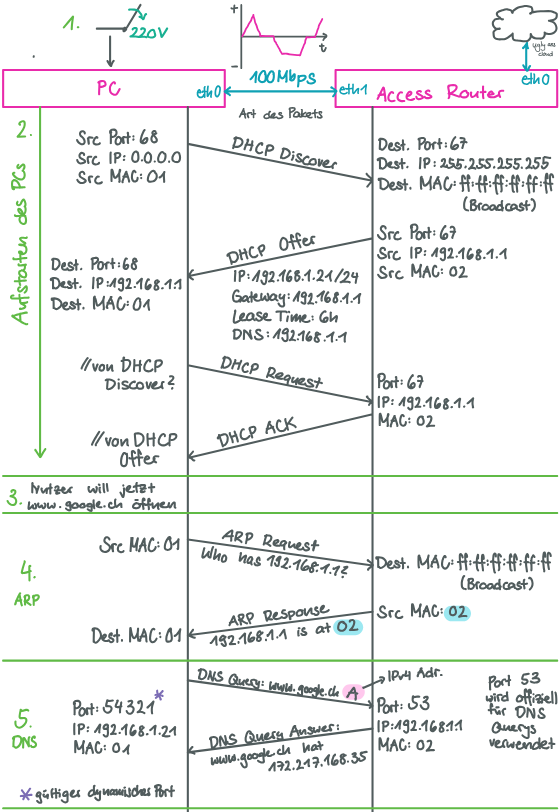
\includegraphics[width=1\linewidth]{images/atoz1.png}\\
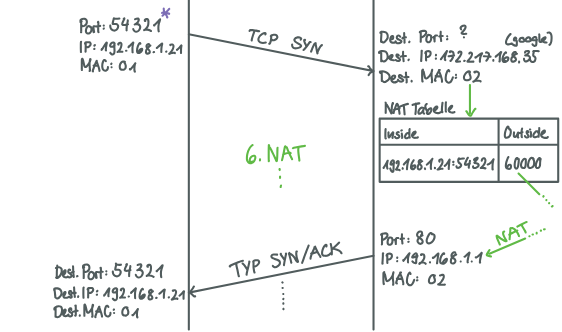
\includegraphics[width=1\linewidth]{images/atoz2.png}



\begin{example2}{Ports{,} Adressen und Routingtabellen} für A-Z Beispiel!\\
    \textcolor{pink}{PC:} UDP-Port = 67, IP = ?, MAC = 01:01:01:01:01:01\\
    Routingtabelle:\\
    \begin{tabular}{|c|c|c|}
        \hline
        Netzadresse + Maske & Port & Gateway\\
        \hline
        192.168.1.0/24 & eth0 & direkt\\
        \hline
        default & eth0 & 192.168.1.1\\
        \hline
    \end{tabular}

    \vspace{2mm}

    \textcolor{pink}{Access Router:} DNS Port = 53, UDP-Port = 67
    \begin{itemize}
        \item Interne IP = 192.168.1.1
        \item Externe IP = 195.1.2.1
        \item MAC = 00:02:02:02:02:02
    \end{itemize}
    Routingtabelle:\\
    \begin{tabular}{|c|c|c|}
        \hline
        Netzadresse + Maske & Port & Gateway\\
        \hline
        192.168.1.0/24 & eth1 & direkt\\
        \hline
        default & eth0 & 195.1.2.1\\
        \hline
    \end{tabular}

\end{example2}


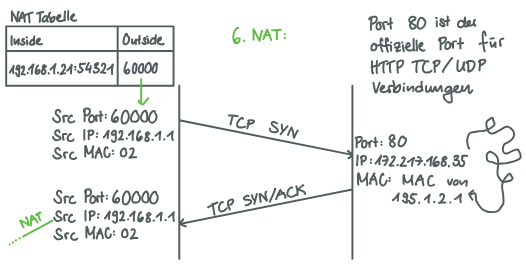
\includegraphics[width=1\linewidth]{images/atoz3.png}



